\documentclass[utf8]{article}


%% Language and font encoding
\usepackage[english]{babel}
%\usepackage[utf8]{inputenc}
\usepackage[T1]{fontenc}

%% Sets page size and margins
%\usepackage[a4paper, top=3cm,bottom=2cm,left=3cm,right=3cm,marginparwidth=4cm]{geometry}
\usepackage[papersize={10in, 12in}, top=3cm,bottom=2cm,left=2in,right=2in,marginparwidth=1.8in]{geometry}


%% Title style
\usepackage{stringstrings}
\usepackage[explicit]{titlesec}
\usepackage{sectsty}



%% ============================== Useful packages ============================= %
\usepackage[dvipsnames,table,xcdraw]{xcolor}
\usepackage[round]{natbib}
\usepackage{amsmath}
\usepackage{graphicx}
\usepackage[colorlinks=true, allcolors=blue]{hyperref}
\usepackage{authblk}
\usepackage{float}
\usepackage{tikz}
\usepackage[threshold=2, autopunct=true, autostyle=true]{csquotes}




%% ================================== acronym ================================= %
\usepackage{acronym}
\newacro{ntic}{non-trivial informational closure}
\newacro{ic}{informational closure}
\newacro{cg}{coarse-grain}
\newacro{cging}{coarse-graining}
\newacro{cged}{coarse-grained}
\newacro{ncg}{neural coarse-graining}


% The name of our theory
% ----------------------------------------------------------------------------
\newcommand{\tnamefull}{The Neural Coarse-graining Theory of Consciousness}
\newcommand{\tname}{NCGT} 	% TheoryNameShort
\newacro{\tname}{\tnamefull}
%\newacro{NCGT}{the neural coarse-graining theory of consciousness}



% =================================== Macro ================================== %
\usepackage[colorinlistoftodos]{todonotes}
\usepackage[at]{easylist}
\usepackage{tcolorbox}
\usepackage{comment}


% Meaning of colours --------------------------------------------------------- %
%	Red: Important and Critical
%	Orange: Todo
%	Blue: Topic and Guideline
%	Purple: Murmur
%	Green: Question, Call for help, Open for opinions and comments
%	Brown: Need Wording
% ---------------------------------------------------------------------------- %


% Real content
	% Finished part
	% Outline items that can be integrated into main text
		\newenvironment{ants}
			{
			 \begin{easylist}[itemize]
		 	}
			{
			\end{easylist}
			}

	% Writing Materials
		\newenvironment{writingMaterials}
			{
			\begin{tcolorbox}[size=small, colframe=black!20!white, toprule=1mm]
				Writing Materials
			\end{tcolorbox}

			\begin{easylist}[itemize]
			}
			{
			\end{easylist}
			\begin{tcolorbox}[size=small, bottomrule=1mm, halign=flush right, colframe=black!20!white]
				Writing Materials
			\end{tcolorbox}
			}

% Functional content
	% Quotes: green
		\newcommand{\rewrite}[1]{\textcolor{ForestGreen}{\textit{"#1"}}\newline}


	% todo: orange
		% text todo
		\newcommand{\toWrite}[1]{\noindent
			\textcolor{Orange}{\textbf{[[ #1 ]]}}}

		% figure todo
		\newcommand{\includegraphicsTodo}[2][]{%
			\tcbox[%
				adjusted title=\LARGE To Be Modified,
				halign title=right,
				colbacktitle=Orange!75!White,
				coltitle=Black,
				colframe=Red!60!White,
				boxrule=1mm,
				colback=white%
				]{\includegraphics[#1]{#2}}}

		% rewording
		\newcommand{\rewording}[1]{\textcolor{RawSienna}{[[ REWORDING | #1 ]]}}

		% Need reference
		\newcommand{\needref}[1]{%
			\ifthenelse{\equal{#1}{}}{%
				\todo[color=White, linecolor=Orange, bordercolor=Orange]{\textcolor{Orange}{Ref}}}{%
				\todo[color=White, linecolor=Orange, bordercolor=Orange]{\textcolor{Orange}{Ref: #1}}%
			}%
		}



	% Highlight
		% Highlight only
		\newcommand{\highlight}[2][Thistle!50!white]{\colorbox{#1}{#2}}

		% Highlight and comment
		\newcommand{\highlightAndComment}[3][Thistle!50!white]{\todo[color=#1]{#3}\colorbox{#1}{#2}}

		% Critical point
		\newcommand{\critical}[1]{%
			\todo[color=OrangeRed!70!white]{#1}
		}




	% idea: Purple
		% text idea
			\newcommand{\idea}[2][Plum]{\noindent
				\textcolor{#1}{[[ #2 ]]}}

		% box idea
			\newcommand{\ideaBox}[1]{
				\begin{tcolorbox}[%
					width=12cm,
					sharp corners=downhill,
					hyphenationfix,
					arc=8pt,
					colback=Thistle!50!white,
					flush right,
					halign=flush right,
					]%
					#1
				\end{tcolorbox}
			}

		% call-out idea
			\newcommand{\ideaCallout}[1]{\todo[color=Thistle!50!white, size=\small]{#1}}


	% communication: green
		% call for help
			\newcommand{\callforhelp}[1]{\todo[color=SpringGreen]{[Call For Help]: #1}}


		% comment
			% comment by authors
			\newcommand{\addcomment}[3][\empty]{\todo[color=SkyBlue]{Comment [#2]:\newline#3}\colorbox{SkyBlue}{#1}}

			% usage:
			% \addcomment{auther}{comment text}
			% or
			% \addcomment[highlighted text]{auther}{comment text}
			%
			% e.g.
			% It's a \addcomment[beautiful]{Acer}{need a reference} day






% ============================================================================ %
%                                     Title                                    %
% ============================================================================ %
\title{A neural coarse graining theory of consciousness}



% ============================================================================ %
%                                    Authors                                   %
% ============================================================================ %
\author[1]{Acer Y.C. Chang\thanks{acercyc@araya.org}}
\author[1]{Martin Biehl\thanks{martin@araya.org}}
\author[1]{Ryota Kanai\thanks{kanair@araya.org }}
\affil[1]{ARAYA, Inc., Tokyo, Japan}



% ============================================================================ %
%                                     Body                                     %
% ============================================================================ %
\begin{document}
	\maketitle
	\tableofcontents


	\begin{abstract}
		Neural systems process information through different levels of organisation in a hierarchical manner. Information at lower levels is finer-grained and can be coarse-grained for higher level computation. However, one is aware of information processed only at specific levels. Theorists have addressed this issue. For example, the intermediate level theory of consciousness suggests that the intermediate level seems to be privileged with respect to consciousness. It is true that we do not experience information processed by individual neurons which is always highly noisy. Besides, we have no conscious experience from interpersonal activities albeit massive interactions among individuals. Instead, neurophysiological evidence has been showing that conscious experience tends to co-vary with information encoded in coarse-grained neural states such as neural population codes. We argue that the neural states within the scope of the informational closure determine the contents of consciousness and brain processes outside apart from the representations of that level remain unconscious. This argument suggests a distinction between conscious and unconscious processing and provides a generic computational framework. Finally, using the deep learning network, we can measure informational closure in deep hidden layers. Our preliminary results show that informational closure representation emerged after learning. We further decoded the information from the representation and compared it with human conscious perception.
	\end{abstract}


	\section*{Keywords:}
	Keywords: theory of Consciousness, informational closure, neural coarse-graining, level of analysis

	% ============================================================================ %
	%                                     Start                                    %
	% ============================================================================ %


	\section{Introduction}

		%% Story about a cell
		Imagine you are a neuron in Alice's brain. Your daily work is to collect neurotransmitters through dendrites from other neurons, accumulate membrane potential, and finally send signals to other neurons through action potentials along axons. However, you have no idea that you are one of neurons in Alice's supplementary motor area and involved in many motor control processes for Alice's action, for example, grabbing a cup. You are ignorant of intentions, goals, and motor plans that Alice has at every moment even though you are part of the physiological substrate responsible for all those actions.
		A similar story also applies to Alice's conscious mind. To grab a cup, for example, Alice is conscious of her intention and visuosensory experience of this action. However, her conscious experience does not show the dynamic of your membrane potential and about action potentials you send to other neurons every second. That is, information in Alice's conscious experience does not contain information involved in your information processing.

		\toWrite{maybe need a transition sentence here}

		%% scale
		It seems to be true that we are unable to consciously access information processed at every scale in the neural system. Only information at certain levels of coarse-graining can become conscious contents. At microscopic levels of neural systems, information processing in individual neurons is highly noisy and state transitions of neurons are extremely stochastic \citep{Goldwyn2011, White2000}. However, instead of stochastic action potentials and fluctuation of random noise at microscopic levels, what we are aware of in our conscious mind shows astonishing stability and robustness against the ubiquitous noise in the neural system \citep{mathis1995computational}. Likewise, conscious experience does not associate with states of the whole brain level because we have known that some parts of the neural system contribute very little to conscious experience (the cerebellum for example \citep{lemon2010life}). Additionally, we do not  experience "super-consciousness" when we have massive inter-individual interactions with other human-beings. Even though evidence has shown several types of collective information processing at human social groups levels exist \citep{malone2015handbook}, information processed at this level seems to depart from our individual conscious contents.


		%% our argument
		In this article, we propose a new theory of consciousness, called\ac{\tname}. This proposal states that consciousness does not rest on particular neural architectures or locations in the neural systems. Instead, we argue that consciousness correlates with information processing at a certain coarse-grained level where the neural systems create a high degree of non-trivial informational closure (NTIC). We further postulate that the \textit{level} of consciousness corresponds to the degree of NTIC and the \textit{contents} of consciousness corresponds to the state of the NTIC process (for the level versus content of consciousness see \cite{laureys2005neural, overgaard2010neural}).


		%% About this paper
		Our theory rests on two core concepts: non-trivial informational closure and neural coarse- graining. In this article, we first introduce non-trivial informational closure and its importance to information processing for human scale agents. We next argue that through coarse-graining the human neural system can achieve non-trivial informational closure at a specific coarse-grained level. We then propose that the state of the informational closure correlates with the state of consciousness for both levels and contents which can be explained, quantified, and predicted computationally by this theory. We also address how this theory can concisely explain empirical results from previous studies and reconcile several current major theories of consciousness. Finally, we provide predictions and testable approaches for this theory.


		% TODO: is figure needed?
		\idea{Do I need a figure?, Something like this one?}
		\begin{figure}[H]
			\includegraphicsTodo[width=\textwidth/2]{WritingMaterials/PDFXCview_2018-06-11_13-37-34.png}
			\cite{pennartz2017consciousness}
			\caption{xxxx}
	   	\end{figure}



		%% backup point
		\begin{comment}
			@ consciousness is information

			@ conscious contents
				@@ \toWrite{lower level}
				@@ Information processing of individual neurons are noisy.
				@@ We don't have conscious content changes when individual neurons fire action potentials.
				@@ Don't even mention ion channel dynamic.


				@@ \toWrite{Higher-level dynamic}


			@ For human, physics at our body scale are nearly follow classic physics, which is deterministic.


			@ \toWrite{Human tendency for active prediction }
				@@ \cite{Stahl2015} \rewrite{
					Given the overwhelming quantity of information available from the environment, how do young learners know what to learn about and what to ignore? We found that 11-month-old infants (N = 110) used violations of prior expectations as special opportunities for learning. The infants were shown events that violated expectations about object behavior or events that were nearly identical but did not violate expectations. The sight of an object that violated expectations enhanced learning and promoted information-seeking behaviors; specifically, infants learned more effectively about objects that committed violations, explored those objects more, and engaged in hypothesis-testing behaviors that reflected the particular kind of violation seen. Thus, early in life, expectancy violations offer a wedge into the problem of what to learn.}

			@ Intuitive physics \needref{Intuitive physics}

		\end{comment}







	\section{Non-trivial informational closure}
		\ideaBox{I am still not sure we should go for NTIC without describe my intuition about consciousness and closure? Or we should start with my intuition. Or we should postpone to explain the intuition in Chapter 4?}

		The notion of non-trivial informational closure (NTIC) is introduced by \cite{BERTSCHINGER.2006}. The concept of closure is closely related to system identification in systems theory. One can define a system from its environment by computing the closureness of the system \citep{maturana1991autopoiesis, rosen1991life, pattee2012evolving, luhmann1995probleme}. The closureness can be further quantified by information theory.

		\begin{writingMaterials}
			@ Consciousness as an intrinsic information. Therefore, information should be self-define. This means the boundary of conscious content should be related to informational closure.

			@ \idea{should we describe the intuition of boundary problem here?}

			@ ============================================================================


			@ \rewrite{
				The notion of closure plays a prominent role in systems theory where it is used to identify or define the system in distinction from its environment} \cite{BERTSCHINGER.2006}

			@ \rewrite{
				Our theoretical interest concerns the type of system that is a unity for and by itself and not only for an external observer distinguishing some entity from the rest of the world. This requires a system that can be described as a whole without reference to its environment. In systems theory, this property is usually referred to as closure.}\citep{BERTSCHINGER.2006}

			@ \rewrite{
				These concepts of closure play an important role in the architecture of systems
				theory, because they are used to
				1. define the system (in distinction to its environment) and to
				2. explain the autonomy of the system.}\citep{BERTSCHINGER.2006}

			@ \rewrite{
				Informational closure: The higher process is informationally closed, i.e., there is no information flow from the lower to the higher level. Knowledge of the microstate will not improve predictions of the macrostate.} \citep[p. 4]{PFANTE.2014}


		\end{writingMaterials}


		% Definition of informational closure
			\noindent
			Information flow $J_{t}$ from the environment $E$ to a system $Y$ at time $t$ can be defined as the conditional mutual information $I$ between the system future state $Y_{t+1}$ and the current environment current state $E_{t}$ given the current system state $Y_{t}$

				\begin{equation}\label{eq:InformationFlow}
				\left.\begin{array}
				{rl}{J_{t}(E \rightarrow Y )} & {:= I(Y_{t+1};E_{t}|Y_{t})} \\
				%{ } & { \ = H(Y_{t+1}|Y_{t})-H(Y_{t+1}|Y_{t},E_{t})} \\
				%{ } & { \ = H(E_{t}|Y_{t})-H(Y_{t}|Y_{t},Y_{t+1})} \\
				%{ } & { \ = H(E_{t}|Y_{t})-H(E_{t}|Y_{t},Y_{t+1})}\\
				{ } & { \ = I(Y_{t+1};E_{t}) - (I(Y_{t+1};Y_{t})-I(Y_{t+1};Y_{t}|E_{t}))}
				\end{array}\right.
				\end{equation}

				\begin{figure}
					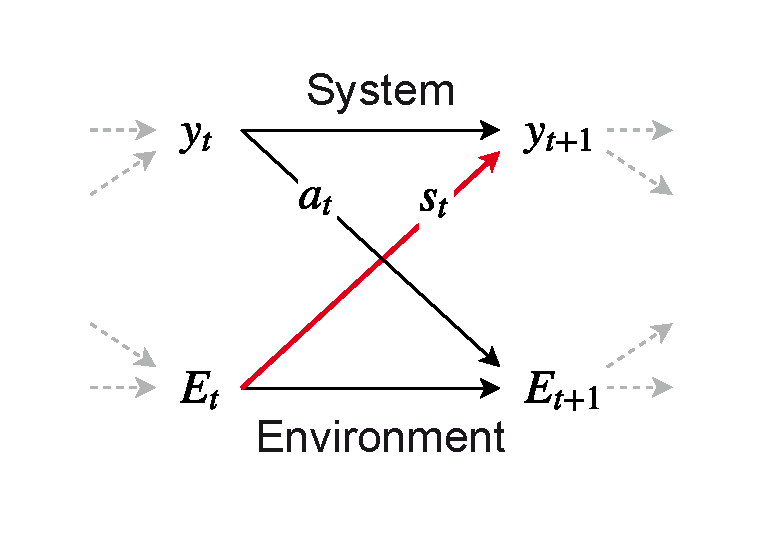
\includegraphics[width=\textwidth]{WritingMaterials/SystemAndEnv.pdf}
					\caption{Figure adapted from \cite{BERTSCHINGER.2006}}
					\label{fig:SystemAndEnv}
				\end{figure}


			\noindent
			\cite{BERTSCHINGER.2006} defines that a system is informational closured when information flow from the environment to the system is close to zero.

				\begin{equation}
				J_{t}(E \rightarrow Y )=0
				\end{equation}


			% ------------------------------- trivial case ------------------------------- %
			\noindent
			Achieving information closure (minimising $J_t$) could be trivial, which means the environment and the system are entirely independent of each other.

				\begin{equation}
				\begin{aligned}
				{I(Y_{t+1};E_{t})=0}&&{\Rightarrow}&&{J_{t}(E \rightarrow Y )=0}
				\end{aligned}
				\end{equation}


			% -------------------------------- non-trivial ------------------------------- %
			\noindent
			However, informational closure can be achieved non-trivially. In the non-trivial case, the system trying to encode information about the environmental dynamics can also be informational closured. This means

				\begin{equation}
				I(Y_{t+1};E_{t}) > 0
				\end{equation}

			\noindent
			This also implies
				\begin{equation}
					I(Y_{t+1};Y_{t})-I(Y_{t+1};Y_{t}|E_{t}) > 0
				\end{equation}



			\noindent
			And, non-trivial informational closure can be defined as
				\begin{equation}
				\left.\begin{array}
				{rl}{NTIC} & {:=I(Y_{t+1};Y_{t})-I(Y_{t+1};Y_{t}|E_{t})}\\
				{ } & {\ =I(Y_{t+1};E_{t})-I(Y_{t+1};E_{t}|Y_{t})}
				\end{array} \right.
				\end{equation}


			\noindent
			And, Maximising NTIC is equivalent to
				\begin{equation}\label{eq:nticObjective}
				\begin{aligned}
				& \text{maximise} & { } & I(Y_{t+1};Y_{t}) & { } & \text{and} \\
				& \text{minimise} & { } & I(Y_{t+1};Y_{t}|E_{t}) & { }
				\end{aligned}
				\end{equation}

			\noindent
			This implies the system contains in itself the information of its own future and the self-predictive information is gained from the information about the environment. Therefore, to achieve NTIC, the system can internalizes and synchronises the dynamics of the environment, i.e. modelling the environment. Furthermore, having high degrees of NTIC entails having high predictive power about the environment. This gives biological agents a great functional and evolutional advantage to achieve NTIC in their information processing systems. Practically, \cite{guttenberg2016neural} proposed that NTIC can be achieved by maximising the predictive power about the environment and the self-predictive information of the system concurrently.


			% Biological evidence of informational closure in the neural system
			Though the significant advantage for biological systems to achieve NTIC, to our knowledge, studies directly examining NTIC in biological systems are limited. However,  recent studies have showed relevant properties in the visual system of salamanders. By examining the salamander retina, in two studies \citep{Palmer2015, sederberg2018learning} the authors found that the a large groups of neural populations of retinal ganglion cells encoded predictive information about external stimuli also had high self-predictive information about their own future states (see Figure~\ref{fig:sederberg2018learning}), therefore, in line with the characteristic of NTIC. Therefore, the self-predictive information of the neural populations can guides prediction about external stimuli without reference to stimulus parameters explicitly. Moreover, the internal predictability can be generalised to different stimulus classes suggesting the tendency to internalise the information of environmental dynamics in the neural populations. \toWrite{Add Some ending sentences}

			\begin{figure}[H]
				\includegraphicsTodo[width=\textwidth]{WritingMaterials/Palmer2015.png}
				\caption{Figure adapted from \cite{sederberg2018learning}}
				\label{fig:sederberg2018learning}
			\end{figure}

			\begin{comment}
				@ ===

				@ \rewrite{
					Internal information reflects the spatial and temporal correlations in the stimulus.}

				@ \rewrite{predictive information is encoded synergistically.}

				@ \rewrite{
					in recordings of populations of RGCs of salamander retina driven by a simple stimulus with partially predictable dynamics, joint activity patterns transmit information that is predictive of future stimuli }

				@ \rewrite{
					We examined whether the temporal correlations within populations of RGCs can be used to guide the search for readouts of predictive information.}

				@ \rewrite{
					We showed that groups of cells with high external, stimulus-predictive information also had high internal predictive information on two classes of stimuli, }

				@ \rewrite{
					Very simple learning rules could find near-optimal readouts of predictive information without any external instructive signal. This suggests that bottom-up prediction may play an important role in sensory processing}

				@ \rewrite{
					Internal predictive information can guide stimulus prediction without explicit reference to stimulus parameters.}

				@ \rewrite{
					Word–word internal predictive information is correlated with word–stimulus predictive information across sets of four cells.}

				@ They also showed generalization of internal predictability across stimulus. This suggests .... what?

				@ \rewrite{
					The generalization of internal predictability across stimulus classes partially reflects the ability of the retina to adapt to the statistics of stimuli}


				@ \cite{Palmer2015}
				@ \rewrite{
					Groups of cells in the retina carry information about the future state of their own activity, and we show that this information can be compressed further and encoded by downstream predictor neurons that exhibit feature selectivity that would support predictive computations.}

				@ \rewrite{
					It seems natural to phrase the problem of prediction in relation to the visual stimulus, as in Fig. 3, but the brain has no direct access to visual stimuli except that provided by the retina. Could the brain learn, in an unsupervised fashion, to predict the future of retinal outputs? More precisely, if we observe that a population of retinal ganglion cells generates the word w t at time t, what can we say about the word that will be generated at time t + Δ t in the future? The answer to this question is contained in the conditional distribution of one word on the other, P ð w t +Δ t j w t Þ } \url{http://tinyurl.com/y9zmhlln}

				@ \rewrite{
					larger groups of cells carry predictive information for hundreds of milliseconds, }



			\end{comment}



			%% backup
			\begin{comment}
				@ Accurately model deterministic environment
				@ \rewrite{
					This demonstrates that a system exhibiting certain internal regularities as measured by $A^* = MI(Sn+1; Sn)$ can achieve informational closure either by gaining information about the environment or by increased autonomy, i.e. by becoming unpredictable or uncontrollable from the (13) environment. Therefore, information about the environment, i.e. modeling, and autonomy can be considered as complementary strategies for achieving informational closure.}

				@ By Action

				@ In the next section, we claim that the neural system achieve NTIC through coarse-graining.
			\end{comment}



		\subsection{Informational closure and level identification \ideaCallout{maybe not necessary}}


		\subsection{Biological Creature may try to achieve closure even the environment is not \ideaCallout{Maybe not necessary}}



	\section{Neural coarse-graining}

		%% stochasticity at microscopic levels
		Nevertheless, to achieve information closure (so as NTIC) in highly stochastic systems (e.g., the neural system) is challenging. The current states of the system have low predictability of its future states due to the stochasticity. Information processing in the neural system is suffered from multiple noise sources throughout, including sensory, cellular, electrical, and synaptic noises. Previous studies have shown that states of neurons have large trial-to-trial variability at the cellular level. That is, the same pattern of activity never occurs twice even when the same stimulus is presented. Neurons are inevitably subject to thermal fluctuations and other physical noises \citep{faisal2008noise}. Furthermore, environmental information is always only partial observable to individual sensors and neurons which only receive little amount of information from the environment. Therefore, self and environmental predictive information is difficult to be represented at the cellular level. It is implausible to construct NTIC processes at microscopic levels.

        %% Our argument
		However, we argue that, by coarse-graining microscopic neural states, the neural system is able to achieve NTIC at certain coarse-grained macroscopic levels. To encode information in coarse-grained variables is a way to encode stable and robust information in neural system and overcome the difficulties to achieve NTIC at microscopic levels. Coarse-graining in this paper is referred to many-to-one functions that map microscopic states to macroscopic states.\needref{Do we need reference?}. In other words, a number of different micro-states realise the same value of the macro-variable \citep{price2007causation}. This is a common strategy that we can see in large number of previous neurophysiological studies. For example, in the temporal domain, neural spikes across time can be coarse-grained as spiking rate variables, known as rate coding \citep{adrian1926impulses, gerstner2002spiking, maass2001pulsed, panzeri2015neural, stein2005neuronal}. Neurons encode stimulus intensity by increasing or decreasing firing rate. \citep{kandel2000principles}. In this coding scheme, individual neural spikes in a transient time span is not meaningful and stochastic \citep{stein2005neuronal}. In contrast, rate codes are relative stable and are highly robust against noise causing variation of inter-spike intervals. 
		
		% population code
		Another example of coding strategy using coarse-graining is population coding. In this coding scheme, information is represented by joint spatiotemporal activities of several neurons. Therefore, the information is encoded in coarse-grained variables whose values are jointly determined by neural activation patterns within a neural population \citep{kristan1997population, pouget2000information, binder2009encyclopedia, QuianQuiroga2009}. In such case, activities of every single neuron is not informative and stochastic. Instead, coarse-grained variables (such as population averaging and population vector) are able to represent information stably. Encoding information at coarse-grained levels allow the neural system ignores certain causal interactions relevant to fine-grained level of description \citep{Woodward2007-WOOCWA}.
			
			
		% neural coarse-graining by Nic
		It has been empirically implemented that NTIC can be achieved by coarse-graining snesory inputs in artificial neural networks. \citep{guttenberg2016neural} proposed a "neural coarse-graining (NCG)" architecture (fig.\ref{fig:NCG}) which aims to captures the emergent large-scale dynamics in the environment. The NCG network learns to coarse-grain input signals and extract latent parameters which are both predictive and predictable in the input signal and therefore achieves NTIC by building a higher-level representation of the underlying dynamics in the deep layers. More importantly, using this architecture, agents can process information and act at coarse-grained macroscopic levels.
		
		\begin{figure}
			\includegraphicsTodo[width=0.8\textwidth]{WritingMaterials/PDFXCview_2018-06-08_14-24-03.png}
			\caption{NCG \idea{I need to simplify this figure}\citep{guttenberg2016neural}}
			\label{fig:NCG}
		\end{figure}		
		

		%% not monotonic
		It is important to note that NTIC should not be a monotonic function of scale of coarse-graining. Overly coarse-graining system states can lead to low degrees of NTIC. For example, in an extreme scenario, when all microscopic states map to a single macroscopic variable, the macroscopic level does not have enough information capacity and thus losses  the self and environmental predictive power. This notion is also supported by empirical evidence. \cite{sederberg2018learning} showed that the efficiency of reading out  self-predictive information of neural population is higher when cell number in populations is 4 than 7 and 10-cell sets. This implies an optimal coarse-graining scale for NTIC processes. % Perhaps the best way to combine more than four cells is to break down the readout into indivisible units of four cells, which are later recombined in subsequent processing.}\citep{sederberg2018learning}


        %% Link to consciousness
        
        At the physical scale which human being live in, the environmental dynamics is nearly deterministic following the laws of classical physics. It gives agents living at this physical scale great advantages if the agents can build NTIC process internally. Therefore, to coarse-grain microscopic states is necessary 
        
        %This means that it is possible for agents to live at this physical scale to build NTIC process internally.
        % More importantly, the information processing related to consciousness should not be situated at this level. Otherwise our conscious percept should be very noisy and unstable.
        



		\begin{writingMaterials}
			@ \rewrite{
				Coarse-graining: a method of reducing the complexity of a system by treating groups of atoms/molecules as single quasi-particles CG: coarse-grained}

			@ neural system use population coding and temporal coding to fight against noise.


			@ Therefore, even though the low level information processing is noisy, it is possible that the neural system achieve NTIC at a coarse-grained level.

			@ This implies that the information about the environmental dynamic should be represented at a certain coarse-grained level rather then other levels.



			%% Macroscale Deterministic
			@ The environment that human scale agents interact with is approximately govern by Newton's law and therefore the state transitions are nearly deterministic.\callforhelp{Is there any good ref I can cite?}

			@ \idea{Need something here}


			%% coarse-graining is necessary
			@ Hence, to coarse-grain states of microscopic levels is necessary to represent and model the human-scale environment state and dynamics.

			@ Coarse-graining is necessary to resist noise

			@ \rewrite{ The population will therefore be relatively insensitive to the loss of
				cells or noise in a small number of cells} \cite{eurich2000multidimensional}


		\end{writingMaterials}


		\begin{comment}


			@ Studies have shown that coarse-graining is a common way that the neural system cope with inevitable noise at microscopic levels.

			@ \rewrite{Because the sequence of action potentials generated by a given stimulus varies from trial to trial, neuronal responses are typically treated statistically or probabilistically}


			@ Note that, information processing related to consciousness should not be situated at this level. Otherwise our conscious percept should be very noisy and unstable.

		\end{comment}


			\begin{writingMaterials}
				@ Population coding

					@@ review ref

						@@@ \cite{Stanley2013}

						@@@ \cite{QuianQuiroga2009}

					@@ \rewrite{
						Averaging is used in many neural systems in which information is encoded as patterns of activity across a population of neurons that all subserve a similar function (for example, see REFs 140,141 )}
										140. Georgopoulos, A., Schwartz, A. \& Kettner, R. Neuronal population coding of movement direction. Science 233, 1416–1419 (1986). 141. Lee, C., Rohrer, W. H. \& Sparks, D. L. Population coding of saccadic eye movements by neurons in the superior colliculus. Nature 332, 357–360 (1988).

					@@ \rewrite{
						Electrophysiological studies in the monkey have shown that behaviourally relevant signals are averaged not only across neuronal populations but also over time in the formation of a behavioural decision 156 .} 156. Gold, J. I. \& Shadlen, M. N. Representation of a perceptual decision in developing oculomotor commands. Nature 404, 390–394 (2000).


					@@ \rewrite{A distributed representation of information of this type is more robust to the effects of noise.}



					@@ \rewrite{
						Neural population code: the set of response features of a population of neurons that carry all information about the considered stimuli. These features consist of spatio-temporal sequences of action potentials distributed across neurons and/or time.}

					@@ The diverse response selectivity of sensory neurons

					@@ \rewrite{
						How a neural population represents information is partly determined by the diverse selectivity of individual neurons \cite{Shamir2014}}



				@ sensory hierarchy
					@@ sensory hierarchy also shows characteristic of coarse-graining


					@@ Due to partial information that sensors can receive

					@@ To form complex representation like shape, objects, coarse-graining is necessary.


					@@ Through coarse-graining, \highlightAndComment{higher level}{might be confusing, need to think about the terminology here} cortical areas can integrate those partial information to infer hidden causes.

			\end{writingMaterials}


			\begin{comment}
				@ Achieving NTIC is the key objective to to extract out latent control parameters in the environment.

				@ Through two objectives during training, the model can achieve NTIC.

				@ this can be achieved by maximising the self-predictive power of deep layers and its entropy through all training data.

				@ With the objectives, NCG network learns to coarse-grain input signals and  extract latent parameters which are both predictive and predictable in the input signal and therefore achieves NTIC by building a higher-level representation of the underlying dynamics in the deep layers.

				@ Agents can process information and act at abstract levels
			\end{comment}


			\begin{comment}
				@ At the physical scale which human being live, the environmental dynamics is nearly deterministic following the laws of classical physics. This means that it is possible for agents living at this physical scale to build NTIC process internally.

				@ When the information in individual sensory channel is noisy and partial, coarse-graining becomes necessary for achieve NTIC.
			\end{comment}




	\section{A neural coarse graining theory of consciousness}
	
	    \subsection{reasoning about this idea}
		\begin{ants}
	    % Intuition
		    
			@ Through coarse-graining, we can define a new set of variables.

			@ If the new set of variables are informational closured, then this creates a new "reality" for all the variables inside.

			@ Reality means the all the information (include variables and the relationships) within the boundary of causal or informational influence between variables.

			@ This is the same as "if a tree falls in a forest" thought experiment.

			@ Therefore, to understand this system, you don't need more information from external environment.

			@ It also means everything in this system is self-defined.


		% Reasoning

			@ Information processing in the neural system exists at different level of abstraction.

			@ The physical environment dynamic at the human scale are nearly deterministic.\needref{Do we need ref here?}

			@ To maximise fitness for individual human-being, neural system should try hard to infer and model the deterministic physical rules.

			@ This drives the neural system to create a non-trivial informational closure.

			@ \idea{okay, I need to be very careful about the causal relation here.}

			@ Therefore, coarse-graining becomes necessary because every individual sensor and neuron at the microscopic scale can only access and process a small part of information.

			@ However, at a macroscopic scale, information processing can achieve non-trivial informational closure (Fig. \ref{fig:CGandIC})


        % our claim   
			@ We claim that the state of a coarse-grained scale which realises non-trivial informational closured correlates the state of consciousness.

			@ We further postulate that level of consciousness corresponds to informational closureness of processes.

			@ The contents of consciousness correspond to the states of the non-trivial informational closure.

			@ \critical{I need to somehow acknowledge \cite{pennartz2017consciousness}}
				@@ \rewrite{ In conclusion, for a well-behaved representational system, it does not matter whether a neural activation pattern represents an external world feature truthfully or not, as long as the system represents the feature consistently over time and in sensory space.}

				@@ pennartz levels are defined by functional elements call "functional ensembles". \cite{pennartz2017consciousness} \rewrite{This delineation is different from a scale-based distinction of levels, because different levels are distinguished here based on function , i.e., what each level can accomplish in terms of computation and representation, culminating in perception at the highest level.}
				
		% Following
			@ In the following part, we....\todo{todo}


		\end{ants}



		\begin{figure}[H]
			\includegraphicsTodo[width=\textwidth]{CGandIC.png}
			\caption{informational closure through neural coarse-graining}
			\label{fig:CGandIC}
		\end{figure}


		% ==================================== %
		% Backup
		% ==================================== %
		\begin{ants}

			@ \rewrite{
				Multilevel views on consciousness and cognition have been expressed before by many other theorists, such as Oppenheim and Putnam (1958), Attneave (1961), Hofstadter (1979, 1985), Churchland and Sejnowski (1992), Wimsatt (1994), and Lycan (1996).} \cite{pennartz2017consciousness}

				@@ Oppenheim , P. , \& Putnam , H. ( 1958 ). Unity of science as a working hypothesis . In H. Feigl , G. Maxwell , \& M. Scriven (Eds.), Concepts, theories, and the mind – body problem (pp. 3 – 36 ). Minneapolis : University of Minnesota Press .
				@@ Attneave , F. ( 1961 ). In defense of homunculi . In W. A. Rosenblith (Ed.), Sensory communication (pp. 777 – 782 ). Cambridge, MA : MIT Press .
				@@ Hofstadter , D. R. ( 1979 ). Godel, Escher, Bach, an eternal golden braid . New York : Basic Books .
				@@ Churchland , P. S. , \& Sejnowski , T. J. ( 1992 ). The computational brain . Cambridge, MA : MIT Press .
				@@ Wimsatt , W. C. ( 1994 ). The ontology of complex systems: levels of organization, perspectives, and causal thickets. Canadian Journal of Philosophy , 20 , 207 – 274 .
				@@ Lycan ,  W. G.  ( 1996 ).  Consciousness and experience .  Cambridge, MA :  MIT Press

			@ It's important that not the neural states but the coarse-grained state determine contents of consciousness.

			@ Consciousness is information
				@@ Information is level-dependent.

				@@ Information is different at microscopic and macroscopic levels

				@@ Consciousness must be level-dependent


			@ \rewrite{
				This illustrates how coarse-graining allows the formulation of incomplete generalizations that are relatively invariant, although at the cost of predictive precision regarding fine-grained details.} \cite{price2007causation}

				@@ conscious perception are very stable and time invariant.
				@@ Conscious perception is informative but we loss all the precise information about the states at microscopic level.
		\end{ants}
		% ==================================== %










		\subsection{Measure of consciousness/information correlate of consciousness}	
		
			\begin{ants}
			
				
			@ In this framework, we postulate that the NTIC process is the core entity of information correlate of consciousness. 
			
			
			@ The content of consciousness corresponds to the state of the NTIC process.
				\begin{equation}\label{eq:cContent}
					C_{t}^{Content} = Y_{t}
				\end{equation}		
				
			@ Furthermore, we can compute the level of consciousness via knowing the amount of information enclosed in a NTIC process. 						
			
			@ We postulate that levels of consciousness $C_{t}^{Level}$ corresponds to the degree of NTIC at the coarse-grained level $NTIC_{t}$ at time $t$.
			
				\begin{equation}\label{eq:cLevel}
					C_{t}^{Level} = NTIC_{t}
				\end{equation}
				
			
			@ Therefore, this framework well integrates the two key but debated concepts in consciousness research \citep{laureys2005neural, bayne2016there}. 
			
			

			\subsubsection{consicous level}
			@ This implies that, based on the Equation \ref{eq:nticObjective}, the self-predictive information about the future states that the current state holds and the information about the environment encoded in the process determine the level of consciousness.
			
			@ This also suggests that the richness of the environment being modelled by the			NTIC process has a direct contribution to the level of consciousness.
			
			
		
			\end{ants}
			
			
			
			
			\begin{writingMaterials}

				@ Based on Equation xxx\todo{equation}, the measure of non-trivial informational closure can be decomposed to XXX and XXX.

				@ use 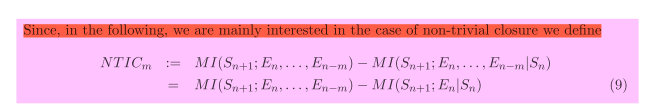
\includegraphics{WritingMaterials/PDFXCview_2018-06-01_17-44-30.png}

				@ or use 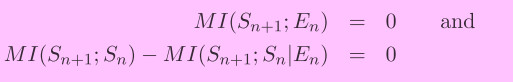
\includegraphics{WritingMaterials/PDFXCview_2018-06-04_19-18-12.png}

				@ To have high level non-trivial informational closure, the states of the coarse-grained scale need to

				@ First, maximise the mutual information between environment and the representation.
				This term implies that the agent need to maximise predictive power of environmental state. This also suggest that the environmental complexity is a crucial factor to the level of consciousness. The more rich and complex environment the agent try to predict the higher level of consciousness the agent has.


				@ Second, to minimise the mutual information between environment and the representation conditional on the past state of the representation. This term suggests that the representation is self-predicable and it mimics the environmental transition.

				@ Therefore, this theory predicts that level of consciousness determined by the environment that the agent adapts to. To form a high non-trivial informational closure, the agent will need to live in a complex environment and model the environmental transition precisely.

				@ \rewording{Note that, our claim is that informational closure is a more fundamental property that correlates consciousness. A species acquiring advantage to model a complex environment through evolution and , therefore, achieving a high-level non-trivial informational closure has a high level of consciousness, is the consequence of the evolutional process. }


			\end{writingMaterials}



		\subsection{Coarse-graining states correlates conscious contents}
			\begin{ants}
				@ We claim that conscious contents correspond to the state of the informational closure.

				@ \idea{= not sure I want to say this here =}

				@ Consciousness is informative. A conscious percept including volition and intention is a unique state that narrowing down all possible states into one. Therefore, a conscious percept reduces a huge amount of uncertainty.



			@ This is similar to the the \textit{Information} axiom in integrated information theory which claims that 

\textquote[\citep[p. 2]{oizumi2014phenomenology}]{...an experience of pure darkness is what it is by differing, in its particular way, from an immense number of other possible experiences...}


``...an experience of pure darkness is what it is by differing, in its particular way, from an immense number of other possible experiences...''\citep[p. 2]{oizumi2014phenomenology}


				@ This is the same claim as the third axiom called "information" in IIT. \needref{information axiom and need to say more about this.}

				@ ====================================

				@ Note that because the closure is at a coarse-grained scale one state of the informational closure can be mapped to several states at microscopic scale.
			\end{ants}




		\subsection{Sensory hierarchy and neural coarse-graining
			\critical{This is super important. I need to deal with this very carefully. Need to completely rewording}}\label{sec:SensoryHierarchy}



			\begin{figure}[H]
				\includegraphicsTodo[width=0.8\textwidth]{hierarchy.pdf}
				\caption{Coarse-grain and sensory anatomical hierarchies}
				\label{fig:hierarchy}
			\end{figure}


			\begin{figure}[H]
				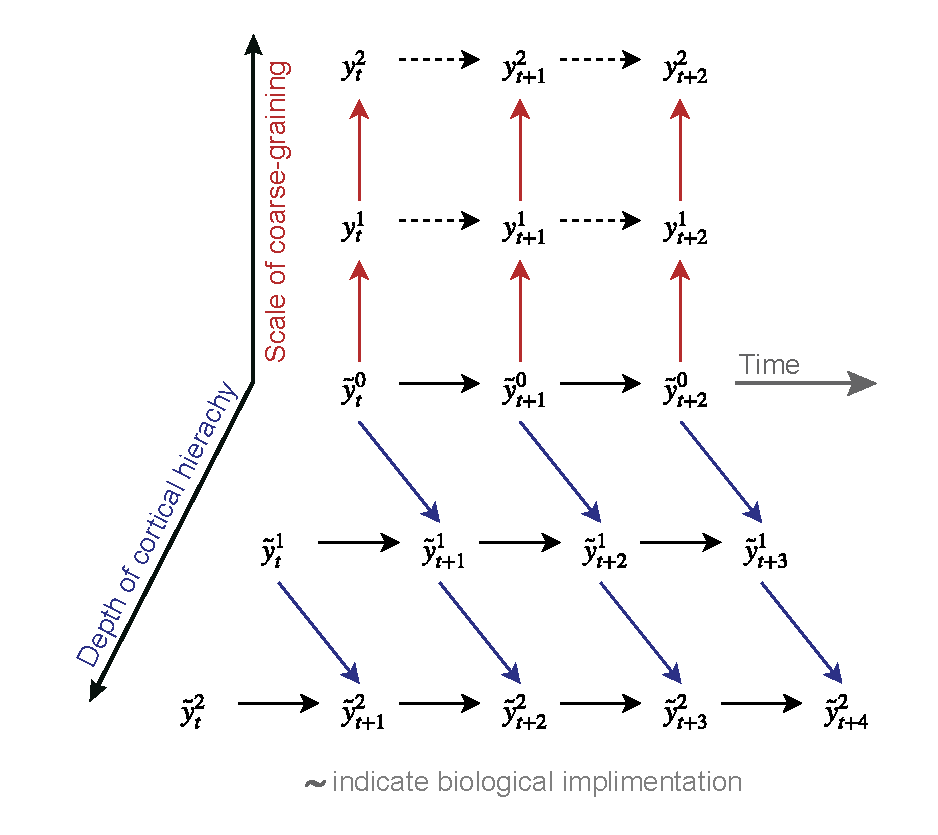
\includegraphics[width=\textwidth]{WritingMaterials/SeperationOfCGandCortHierachy.pdf}
%				{Coarse-grain and sensory anatomical hierarchies}
			\end{figure}




			\begin{ants}
				@ It's important to note that the coarse-graining direction is not necessary to be align with anatomical sensory hierarchy in the neural system.

				@ the coarse-grained information is needed and computed only when the information is required for microscopic scale processing.

				@ \toWrite{I need a strong example here}


				@ Of course, from evolutional perspective, neural system should develop a better hardware to support neural coarse-graining

				@ For example, pooling layers in CNN is an implementation of coarse-graining function. It' is very plausible visual processing hierarchy in the neural system realises pooling layers.


				@ It is possible that the neural system represents higher-level information processing by low level physical subtract. For example, studies have found representation for summery statistics of signal and neural. population.\needref{neural representation for summery statistics}\\
				From this point of view, sensory hierarchy may extend along with levels of coarse-graining.



			\end{ants}






		\subparagraph{more information theory and philosophy relevance}
			\begin{writingMaterials}
				@ One consequence of coarse-graining is that it makes it permissible to ignore certain causal factors that would be relevant at more fine-grained level of description. \cite{price2007causation}

				@ This means the fine-grain variable does not exist at the coarse-grained causal chain.
			\end{writingMaterials}




		% ============================================================================ %
		%                         Information and system theory                        %
		%                                                                              %
		% ============================================================================ %
		\subsection{Information and system theory}
			\idea{A closure can define a system, consciousness is information}

			\idea{Could be linked to system theory, but may need help}

			\rewrite{
				This self-referential distinction from its environment therefore gives rise to the specific autonomy of such a system. Consequently, in systems theory, closure properties and autonomy are considered to be closely related concepts which are both at the heart of defining the system itself.}



		\subsection{Empirical approaches of measuring neural informational closure}



	\section{Conscious vs unconscious processing}
		\ideaBox{Now we can combine "Relation to empirical findings in neuroscience and studies of consciousness" and "About Phenomenology (conscious processing)" in to this}



	\section{Comparison with other theories}
		\ideaBox{Main points should be same/diff, our advantages, and predictions}


		\subsection{Theories about level of abstraction and coarse-graining}
			\begin{ants}
				@ Before the current theory, several theories and perspectives of consciousness have proposed the notion that links level of abstraction or coarse-graining in the neural system to consciousness.

				@ We shortly describe two theories which is \todo{XXX and XXX} related to our current proposal.
			\end{ants}


			\subsubsection{Intermediate Level Theory}
				\begin{ants}
					@ Intermediate Level Theory (ILT) proposes that conscious experience only correlates specific levels of representations in the sensory processing the hierarchy. \citep{prinz2007intermediate, jackendoff1987consciousness}. This theory claims that consciousness only associates with the representation at  intermediate levels rather than the ones at lower-level or higher-level.


					@ A critical difference between ILT and our theory is that our theory doesn't assume the direction of coarse-graining should align with the direction of  anatomical processing levels along cortical hierarchies.
				\end{ants}


				\begin{comment}
					%% Back up materials
					@ \rewrite{
						The intermediate level theory originally proposed by Ray Jackendoff and further defended and specified by Jesse Prinz proposes that within the hierarchy of representations that are used to describe the cognitive system, conscious experience occurs only for specific levels of representation. The theory is rooted in Jackendoff ’s analysis of different cognitive systems such as vision, language, and music and the subsequent observation that consciousness does not arise anywhere within these systems. According to Jackendoff, consciousness is not associated with low-level, nor with high-level representations, but rather with those implying intermediate levels of processing. For instance, in the domain of object recognition, it is assumed that the visual system comprises a low level with local computations of visual features, an intermediate level reflecting binding and object recognition, and a higher level computing viewpoint invariance and representing abstract categories. According to Jackendoff and Prinz, conscious experience is not comprised of a disunified picture of visual features, nor is it represented by viewinvariant categories. Rather it is composed of bound and specific instances of objects that are assumed to be computed at the intermediate level of representation. In an analogous manner, speech perception can be decomposed into three levels: an acoustic representation of speech sounds at the lower level, a high level involving abstract lexical and syntactic categories, and in between a word recognition level relying on phonological representations. This theory explains why the conscious experience associated with speech perception mostly involves phonological representations, rather than other levels of representations. In Jackendoff and Prinz’ theory,the privileged role of the intermediate level of processing is based on the need for real-time computational efficiency. Indeed, this level of representation is assumed to be the most relevant one regarding ecological and functional needs. Another important aspect of this theory concerns the central role of attention during conscious experience. Here, attention is defined as a selection process that acts as a gate to working memory mechanisms. It performs the function of selecting the relevant information that is amplified afterward and then becomes conscious. Indeed, Prinz acknowledges that activation of an intermediatelevel representation on its own cannot be a sufficient condition for consciousness, given that those representations can be activated during subliminal perception. However, this theory makes the crucial postulate that the amplification of intermediatelevel representations by attention is a necessary and sufficient condition for consciousness. In sum, for each domain of processing, the content of consciousness at a particular moment is supported by a representational structure of intermediate level for that domain, which is selected to enter short-term memory, and enriched by attentional processing.} \cite{banks2009encyclopedia}

					@ \rewrite{
						In 1987, Ray Jackendoff published Consciousness and the Computational Mind. In it, he posed an important Where question: Where, in the fl ow of information, does consciousness arise? Most cognitive scientists agree that the mind is, in some sense, a computer. It is a device that processes information by transforming representations in accordance with rules. Computational devices decompose into various interconnected subsystems, each of which performs some aspect of a complex task. Given such a decompositional analysis, we can ask: in which subsystems does consciousness arise? If we depict the mind as a vast fl ow chart, and highlight the boxes whose rules and representations are conscious, which boxes should we mark? Jackendoff ’s answer is simple and elegant. He noticed that many of our mental capacities, including our senses and our language systems, are organized hierarchically. In each of these hierarchies, it makes sense to talk about low- , intermediate- , and high- level processing systems. We break down tasks into stages. Appealing to prevailing models of these stages, Jackendoff observed that the intermediate level seems to be privileged with respect to consciousness. Consciousness seems to arise in intermediate- level processing systems and not elsewhere.} \cite{prinz2007intermediate}

					@ \cite{jackendoff1987consciousness}
					@ \cite{prinz2007intermediate}
					@ 2.5D


					@ about why it is this level
					@@ \rewrite{
						Under the computational interpretation, the “why” question means: In what sense are intermediate level representations computationally important or distinctive? Th is is a tractable question, and it may lead to insights into the function of consciousness. Representations at the intermediate level are ideally suited for real- time deliberative behavioral responses. Low- level representations fail to bind features into coherent wholes. If we are going to interact with our environment, the low level is not a good guide. Th e high level is a good deal better for action, but also suboptimal. Th e high level tells us the category of the stimuli we perceive, but from an allocentric point of view. It abstracts away from stimulus features that are crucial for action. If we encounter a predator, the high- level visual representation does not tell us if it is facing toward us or away from us. Without that knowledge, we cannot decide what course of action to take. So, I propose that the intermediate level plays a distinctive role in information processing. It delivers representations that are coherent but viewpoint specifi c. Th ese representations are useful for determining what to do here and now.arg1} \cite{prinz2007intermediate}
					@@ \rewrite{
						I conclude that the intermediate level plays a distinctive and important computational role. Some researchers fi nd this puzzling. In wondering why the intermediate level is privileged, they note the arbitrariness of the fact that perceptual hierarchies have three levels. Could they not have two? Or a hundred? Do the 50 or so areas that contribute to visual processing really divide neatly into three levels? I think these puzzles depend on a particular understanding of what the word “intermediate” amounts to. One might get caught up in the fact that the intermediate level is the second stage in a sequence. Call this the “serial understanding of the intermediate level.” Alternatively, one might think of the intermediate level semantically. On this reading, the intermediate level is one that is not abstract and categorical, but not piecemeal or disunifi ed. Th ese notions are all in need of some refi nement, but, as a fi rst approximation, the idea is that intermediate- level representations are neither too specifi c nor too general.}\cite{prinz2007intermediate}



					%% Our theory
					@ However, as we mentioned in Section \ref{sec:SensoryHierarchy}, \rewrite{The notion of ‘ levels ’ deployed here is functional and very different from that of successive anatomical processing stages along cortical hierarchies [75] or from anatomic scales in the brain. The multi-level concept in [2] is more akin to Marr ’ s original distinction between the levels of (neural) implementation, algorithms, and computational theory [122], but focuses on how conscious representations correspond to computational operations at levels with lower complexity and representational capacity.}
				\end{comment}


			\subsubsection{The difference between ILT and our theory}
				Prinz suggested that \rewrite{as. Cells in V1 are not promising candidates, because they do not reliably respond in ways that are consistent with features that we experience consciously. } \cite{prinz2007intermediate}

				* Our prediction is, if information that is carried by v1 neurons are necessary to complete informational closure, the states of V1 neurons should also co-vary with conscious contents.

		\subsection{First-order theories}
			\begin{writingMaterials}
				@\rewrite{
					The first-order view maintains that conscious awareness is determined by early sensory activity alone, independently of higher-order representations. Thus the crucial difference between the first-order and higher-order views is that the latter but not the former predict that conscious awareness is determined at least in part by prefrontal and parietal activity. Therefore, in the group of first-order theorists we include here not only those commonly labeled as such in the philosophical literature [11] but also theorists, such as Ned Block [12,13], who hold that the phenomenal qualities of awareness depend on the biological substrate rather than merely the content of the first-order representations, as well as scientists who hold that visual awareness depends on activity in content-specific regions of the extrastriate cortex [24,25] or on feedback from these regions to the primary visual cortex [26]. Most first-order theories explain the difference between awareness and unawareness by positing that the latter is associated with weak information [29] or with representations in alternative (e.g. subcortical) sensory pathways. Thus this view suggests that conscious and unconscious processing will have different functional consequences. Whereas some first-order theorists hold that some higher cognitive functions can be performed without conscious awareness [30–32], most first-order theorists take a difference in perceptual task performance (e.g. ‘hits’ vs ‘misses’ in a detection task) as evidence for a difference in conscious awareness [12,13,25,26,33]. In other words, they typically associate task performance with awareness..} \cite{lau2011empirical}

				@ Among those are first-order theories, on which a mental state is conscious if being in that state results in one’s being conscious of something;


				@  According to first-order views, phenomenal consciousness consists in analog or fine-grained contents that are available to the first-order processes that guide thought and action. So a phenomenally-conscious percept of red, for example, consists in a state with the analog content red which is tokened in such a way as to feed into thoughts about red, or into actions that are in one way or another guided by redness.

			\end{writingMaterials}




		\subsection{Global workspace theory}

			\begin{ants}

				%% Introduction
				@ Global workspace theory (GWT)\cite{baars1988cognitive, baars1997theatre, baars2002conscious} or Global Neuronal Workspace theory (GNWT)\cite{dehaene1998neuronal, dehaene2001towards, dehaene2011experimental} states that the neural system consists of many separate specialised modules and a central global workspace (GW) which integrates and passes information amount the modules. Only the information that is accessed by the global workspace can be conscious aware of. The modules competes with each other to gain the access to the global workspace and the information from the winner can trigger an all-or-none "ignition" in the global workspace and be globally broadcasted to other modules. Conscious contents then associates information which gains access to the internal global workspace \cite{Dehaene2017}.

				%% Our theory

				@ GW in previous data is the place that form NTIC.

				@ non-linearity and emergence

				@ what's the different prediction?

				@ We predict that when the new



			\end{ants}



			\subsubsection{Global availability and Broadcasting}

			\subsubsection{Code translation}
				\begin{ants}
					@ neural coarse-graining can natually solve this problem.
					@ coarse-graining between levels can be thought as code translation\todo{is this true?}
				\end{ants}


			\subsubsection{Stability}
				\begin{ants}
					@ the presence of contexts as stable coalitions shaping access to the workspace.

					@ e ‘all-or-none’ behavior, whereby the incoming evidence either quickly dies out (corresponding to subliminal processing) or is accumulated and amplified non-linearly into a full-blown state of high-level activity. This global ‘ignition’ has been proposed as a marker of conscious perception [70]. Indeed, empirically, when stimulus strength is varied, the early stages of non-conscious processing typically show a linear variation in activation, whereas conscious access is often characterized by a late non-linear amplification of activation which invades a distributed set of parietal, prefrontal and cingulate areas
				\end{ants}


			\subsubsection{Broadcasting}




			\subsubsection{Ignition}
				\begin{writingMaterials}
					@ Conscious access as an accumulation of evidence leading to an all-or-none ignition What, if anything, remains unique to conscious processing? Although many cognitive operations can be partially launched non-consciously, these operations rarely if ever run to completion in the absence of consciousness. A subliminal stimulus may induce above-chance performance, behavioural priming, and a small amount of brain activity in narrowly defined brain networks, but these measures often increase dramatically as soon as the subject reports seeing the stimulus, especially in high-level areas [46 60,61  ]. Accumulation of evidence has been demonstrated with non-conscious stimuli [59], but only conscious stimuli cross the threshold beyond which an overt strategy can be flexibly deployed
				\end{writingMaterials}





			\begin{ants}
				@ GWT is one of the current popular consciousness theories.

				@ \rewrite{AI system and corresponds to our first functional definition of consciousness: global availability} \cite{Dehaene2017}

				@ C1: Global availability of relevant information The need for integration and coordination \cite{Dehaene2017}

				@ Evidence for integration and broadcasting

				@ Stability as a feature of consciousness \rewrite{“ meta-stability ” seems to be necessary for the nervous system to integrate information from a variety of modules and then broadcast it back to them, achieving flexible cross-module routing.}

				@ \rewrite{integration of computational resources in a large-scale coordination and for the exchange of information among processors}

				@ \rewrite{Grounded on the distinction between conscious and unconscious processes, Bernard Baars’ global workspace theory is one of the most influential cognitive theories of consciousness. This theory relies on the metaphor of a theater. In this theater, unconscious specialized processors (equivalent to modules) are assumed to be the actors and the audience. While the audience represents the set of passive processors, actors represents active processors playing on the stage of the theater (i.e., the workspace). These actors are engaged in a competition for being seen by the audience: by broadcasting their information they actually compete for more broadcasting. Active processors with the highest coherent activity can form local coalitions that strengthen them in this competition process. The strongest coalition in this competition dominates the workspace, in a winner-take-all fashion, and corresponds to the content of consciousness. The workspace is equated by Baars to working-memory, in which only the most active content becomes conscious. Additionally, the dominant coalition benefits from global broadcasting, which allows it to recruit new processors from the audience in order to form a global coalition. Here, consciousness allows for the integration of computational resources in a large-scale coordination and for the exchange of information among processors that would otherwise remain separated. In this theory, each processor can operate in the conscious mode if it benefits from global broadcasting through the workspace, or it can operate in the unconscious mode when disconnected from the workspace. An important feature of the global workspace theory is the presence of contexts as stable coalitions shaping access to the workspace. Contexts are constituted of unconscious processors reflecting, in a hierarchical manner, our expectations, our beliefs, our goals, and ultimately our self. In particular, attention is implemented as a goal context in this theory. It is described as a mechanism that controls access to the workspace, acting as a filter and biasing the competition process toward a particular set of actors. At any given moment, the dominant coalition is under the spotlight of attention, and its informational content becomes the content of conscious experience. A crucial aspect of Baars’ theory is that it avoids the problem of the homunculus by reducing it to an audience of multiple unconscious processors. Here, there is no need for a hypothetical single conscious observer in the system, and thus there is no issue of infinite regression with a homunculus inside another homunculus. Instead, consciousness is considered to reflect the global broadcasting of information to an audience of unconscious processors. As the audience is unconscious, unsupervised, and receptive rather than attending to the information, it does not constitute an internal homunculus.}



			\end{ants}






		\subsection{Higher Order Thought theory of consciousness}
			\idea{
				People think a high order representation receives information from the first order representation. This may be a misunderstanding. This may be the result of neural coarse-graining. Because contents in informational closure look like watching fine-grained information, people may have an wrong impression about it}

			============================================================================
			\begin{ants}
				@ Information closure directly is critical for other systems to construct forward models.

				@ Therefore, most of the high level cognition can utilise the state of informational closure.

				@ For example, mental planning needs a precise forward model to infer the environmental dynamics.

				@ \idea{This is way HOT always involve consciousness }

				@ \cite{rosenthal2005consciousness}
			\end{ants}


			\rewrite{
				Higher-order theories of consciousness argue that conscious awareness crucially depends on higher-order mental representations that represent oneself as being in particular mental states.} \cite{lau2011empirical}


			\rewrite{
				According to this view, humans not only have first-order non-conceptual and/or analog perceptions of states of their environments and bodies, they also have second-order non-conceptual and/or analog perceptions of their first-order states of perception. And the most popular version of higher-order perception theory holds, in addition, that humans (and perhaps other animals) not only have sense-organs that scan the environment/body to produce fine-grained representations that can then serve to ground thoughts and action-planning, but they also have inner senses, charged with scanning the outputs of the first-order senses (i.e. perceptual experiences) to produce equally fine-grained, but higher-order, representations of those outputs (i.e. to produce higher-order experiences). A version of this view was first proposed by the British Empiricist philosopher John Locke (1690). In our own time it has been defended especially by Armstrong (1968, 1984) and by Lycan (1996).} \url{https://plato.stanford.edu/entries/consciousness-higher/#SelRepHigOrdThe}

			\rewrite{
				neutral about whether conscious awareness adds significant utility or immediate impact on behavior and task performance [1,27]. This is because the view assumes that task performance in most perceptual and cognitive tasks depends mainly on first-order rather than higher-order representations. Because conscious awareness can differ even if all first-order representations remain completely unchanged, such awareness itself might serve little function [1,27].}\cite{lau2011empirical}
				\ideaCallout{
					My theory would have similar prediction. Because conscious contents are coarse-grained results from low-level information. It is possible that more than two low-level neural states all coarse-grained to a high-level state.  }

			\subsubsection{Metacognition}
				\rewrite{
					Metacognition: cognition that is about another cognitive process as opposed to about objects in the world. In this article we use it mainly to refer to sensory metacognition: a cognitive process that concerns the quality or efficacy of a perceptual process. The capacity of sensory metacognition is sometimes empirically assessed by the correspondence between subjective report and task performance: how closely are they associated with each other on a trial-by-trial basis}\cite{lau2011empirical}



		\subsection{Sensorimotor contingency}
			\begin{ants}
				%% SMC

				@ Sensorimotor contingency (SMC) theory of consciousness is proposed to account of conscious perception. It suggests that different types of SMCs give rise to different characteristics of conscious perception \cite{o2001sensorimotor}.

				@ The theory radically rejects the view that conscious contents is associated with information encoded in internal representations in the neural system.

				@ Rather, the quality of conscious perception depends on agents' mastery of SMCs.

				@ It emphasizes the importance of the interactions between a system (the neural system) and its.

				@ Counter-intuitively, because consciousness inhabits in interactions between agents and environments, this theory suggests that consciousness is not driven by brain activities. Instead, consciousness should be shaped by the way of interaction, i.e. SMCs, between agents and environments.



				%% Our theory

				@ Similar to the SMC theory, our theory predicts that the interaction between the neural system and the environment shapes the quality of conscious perception.

				@ This is because to achieve NTIC the neural system should maximise the conditional mutual information between the future state of the NTIC process and the environment given the agent's current action (see equation XXX \critical{I NEED A EQUATION!}).

				@ This suggests the to maximise NTIC the NTIC process needs to involve the information about the environmental transition and dynamic after agent preforms an action.


				@ Therefore, as a consequence of maximising NTIC, the representation forming NTIC implicitly encodes information about SMCs.

				@ In the long-term, once NTIC neural dynamic interoperates the environmental state transition given actions via maximising NTIC, the state space of XXX then is shaped by the new learned SMC

				@ Accordingly, the way how the agent interacts with the environment influences the structure of the NTIC representation.



				@ \todo{Need to involve some sentence from  }

				@ \idea{Do I need a figure here?}

				@ However, in contrast to the SMC theory, our theory suggests the state of NTIC process correlate conscious contents. Therefore, if the NTIC process is formed inside the neural system, we should have correspondent conscious contents in our conscious experience without interacting with the environment.

				@ \idea{Not sure here} This can easily explain that the conscious experience of dream is just induced by self-evolved state changes of the NTIC process.


				@ Further more the SMC and our theories make complete different prediction about the relationship between SMC and consciousness.

				@ Contrary to the SMC theory which suggests that consciousness resides on SMCs, our theory predicts that pure S-R contingency between the neural system and the environment can not achieve informational closure within the neural system and therefore is not conscious (please see section \ref{sec:reflexive})

			\end{ants}


			\begin{comment} % materials

				%% Intro about this theory
				@ O’Regan and Noë


				@ \rewrite{According to Noë, perceptual presence is explained by a “ sensorimotor theory ” on which perception depends on a practical mastery of sensorimotor dependencies or “ sensorimotor contingencies ” (SMCs) (O ’ Regan & Noë, 2001). The theory inherits from Gibsonian notions of “ affordances ” (Gibson, 1979) and from enactive cognitive science (Thompson & Varela, 2001) which stress the importance of brain-body-world interactions in cognitive processes. On sensorimotor theory, the perception of a tomato as a (perceptually present, real, subjectively veridical) tomato is given by practical mastery of the SMCs governing how the sensory responses elicited by the tomato will behave in a variety of situations. A strong point of this theory is that it suggests why there are differences in qualitative character between modalities, the reason being that different modalities instantiate different SMCs (O ’ Regan & Noë, 2001). }

				@ In their seminal article O’Regan and Noe¨ (2001) introduce sensorimotor contingencies (SMCs) as the basis of a sensorimotor account of conscious perception.

				@ In short, different types of SMCs give rise to different qualities of sensory experience

				@  Second, vision, audition, touch, etc., correspond to domains of knowledge of the respective SMCs that are exercised by an agent as part of its habitual behavior.This ‘‘mastery of SMCs’’ is what lets an agent perceive its environment and adapt its behavior accordingly

				@ And third, sensory awareness arises when SMCs are integrated with planning, reasoning, and generation of behavior

				@ The theory is a radical departure from the classical view that the brain constructs an internal representation of the outside world on which higher cognitive processes such as memorizing, reasoning, and planning operat

				@ perception depends on a practical mastery of sensorimotor dependencies or “sensorimotor contingencies” (SMCs)

				@ s the importance of brain-body-world interactions in cognitive processes. On sensorimotor theory, the perception of a tomato as a (perceptually present, real, subjectively veridical) tomato is given by practical mastery of the SMCs governing how the sensory responses elicited by the tomato will behave in a variety of situations.

				@ ways of acting or as something we do, rather than an internal phenomenal experience or an internal representation of the world (O’Regan \& Noë, 2001)

				@ \rewrite{I advance this truly astonishing hypothesis: To understand consciousness in humans and animals, we must look not inward, into the recesses of our insides; rather, we need to look to the ways in which each of us, as a whole animal, carries on the processes of living in and with and in response to the world around us . . . You are not your brain . . . Meaningful thought arises only for the whole animal dynamically engaged with its environment . . . And indeed the same is true for the quality of our conscious episodes . . . The taste of licorice is not something that happens in our brains.} (Noë, 2009, pp. 7–8)

				@ Because consciousness resides in our behavioural interactions with the world rather than in our brain, the theory postulates that consciousness does not derive from brain activity at all. Consequently, there is no need to explain how brain activity causes or constitutes consciousness, because it does not.

				@ O ’ Regan, J.K. and Noë, A. (2001) A sensorimotor account of vision and visual consciousness. Behav. Brain Sci. 24, 939 – 973

				@ SMC theory argues that consciousness arises from the execution of SMCs, resulting in brain – environmental interactions.

				@ The second variant of SMC theory postulates that ‘ it is not movement as such, but the consequences of potential movement that play a role ’ (in perceptual experience) ([5], p. 1015; see also [9,10,19,20]). This ‘ non-acute ’ or dispositional variant marks a signi fi cant shift in position because it de-emphasizes actual movement. \cite{pennartz2017consciousness}

				@ It stipulates that for us to be conscious of something in the environment (or of our way of interacting with the environment)

			\end{comment}







		\subsection{Predictive Processing}
			\begin{ants}
				%% Introduce PP
				@ The predictive processing is a powerful framework (PP) which integrates several influential ideas in the history of neuroscience including "perception as unconscious inference" from Helmholtz \citet{helmholtz1866concerning}, "analysis by synthesis", “predictive coding”, "Bayesian brain hypothesis"


				@ is a powerful framework


				@ a recent emerged theoretical framework of perception and brain function, which suggests that the brain continuously generates and updates predictions about incoming sensory signals, represents a general principle of neural functioning.


				@ According to predictive processing (PP) account of perception, the neural system constantly performs unconscious statistical inference about hidden causes in the external environment. The perceptual contents are the "best guess" about the environment 	\cite{clark_2013}			\cite{Hohwy2013}

				@ Bperceptual content is the result of probabilistic inference on the hidden causes of sensory signals.


				@ Because it is well integrated with Bayesian brain hypothesis, the PP framework has been used to interpret conscious perception in many perceptual domain. \cite{Hohwy2013} \cite{SethPP2014}



				%% The gaps between pp and consciousness
				@ However, to link PP to consciousness, there are still two major gaps.


					@@ First, previous studies have demonstrated many brain processes following the principle of Bayesian inference and Bayesian integration. But not all these processes are conscious. This indicates that PP is not a sufficient mechanism for conscious perception. Some other factors may be involved to determine which PPs can be conscious or not.


					@@ Second, it has been emphasized that only the results of the inference or prediction can be consciously accessed. The process of inference in completely unconscious. So WHY?

				@ Even though PP has been acquiring attention in different discipline in neuroscience, So far, to our knowledge, no detailed explanation has been given to account for the two questions.




				%% Our theory

				% 2018/06/15 15:10
				@ We first hypothesize that predictive processing stays unconscious is because it is not able to achieve NTIC.

					@@ \idea{Example from PID controller?}

				@ Second, according to our theory, it is obvious that the computation of predictive processing is unconscious and only the result is conscious. Because the computational details is not at the coarse-grained level which achieves NTIC.

					@@ So far, many neuronal models and coding schema have been proposed to explain how to implement Bayesian inference and prediction at the neuronal level.

					@@ However?


				@ We hypothesize that the distinction between conscious and unconscious predictive mechanisms is whether they build up on the information from the NTIC process.





			\end{ants}




			\begin{writingMaterials}

				%% About the unconscious Bayesian processing
				@ \cite{lamme2015predictive}
					@@ To my knowledge, this is the first time this has been so explicitly laid out—writers on predictive coding thus far have always stayed a little vague on where exactly consciousness sits in the Bayesian framework.

					@@ Yet the two points seem contradictory. In the Bayesian predictive coding framework, consciousness is the result of the unconscious inferential processes.


					@@ However, these authors have so far been very reticent about how exactly consciousness fits into the PC framework. For now, there is an emerging idea that understands consciousness as the final result of unconsciousness processing. According to Hohwy (2013), perceptual consciousness fits in the PC theory as the ‘upshot’ or ‘conclusion’ of unconscious perceptual inferences. Melloni (2014) also expects that inferential processes are conducted behind the curtain of consciousness and what we experience are the ‘outcomes’ or ‘results’ of an unconsciou inferential process. Lamme (2015) agrees with the idea that consciousness is based on the relation or more precisely conjunction of current inputs and priors, which together produce posterior beliefs. Karl Friston agrees to a certain extent with this interpretation of consciousness. According to Hobson and Friston (2016), consciousness is not a phenomenon but a process, a process of optimizing beliefs through inference (consciousness, dreams, and inference; the Cartesian theater revisited; a response to our theater critics).


				@ Link PP and c
					@@ \cite{hobson2016response}
					@@ \cite{Melloni2015}

				%% ----------------------------------------------------------------------------
				@ \cite{SethPP2014}

				@ When uncertainty is high, we should expect an increase in the ability of ever higher-level prior beliefs to determine conscious experience. I

				@ determine conscious experience.

				@ PP combines and builds upon previous ideas about the role of “unconscious inference” in perception (Helmholtz, 1925; Barlow, 1961; Gregory, 1970), the process of “analysis by synthesis” in psychology (Neisser, 1967), the “predictive coding” approach in neuroscience (Srinivasan et al., 1982; Rao and Ballard, 1999; Huang and Rao, 2011) and “generative models” and related probabilistic computational principles (MacKay, 1956; Mumford, 1992; Dayan et al., 1995; Hinton, 2007a,b; Tenenbaum et al., 2011).


				@ \rewrite{The brain is constantly confronted with a wealth of sensory information that must be processed efficiently to facilitate appropriate reactions. One way of optimizing this processing effort is to predict incoming sensory information based on previous experience so that expected information is processed efficiently and resources can be allocated to novel or surprising information. Theoretical and computational studies led to the formulation of the predictive coding framework (Friston 2005, Hawkins and Blakeslee 2004, Mumford 1992, Rao and Ballard 1999). Predictive coding states that the brain continually generates models of the world based on context and information from memory to predict sensory input. In terms of brain processing, a predictive model is created in higher cortical areas and communicated through feedback connections to lower sensory areas. In contrast, feedforward connections process and project an error signal, i.e. the mismatch between the predicted information and the actual sensory input (Rao \& Ballard, 1999). The predictive model is constantly updated according to this error signal. }




				@ \rewrite{Predictive inference and perception The concept of PC overturns classical notions of perception as a largely ‘bottom-up’ process of evidence accumulation or feature detection, proposing instead that perceptual content is specified by top-down predictive signals that emerge from hierarchically organized generative models of the causes of sensory signals. According to PC, the brain is continuously attempting to minimize the discrepancy or ‘prediction error’ between its inputs and its emerging models of the causes of these inputs via neural computations approximating Bayesian inference (Figure 1 and Box 1). Importantly, prediction errors can be minimized either by updating generative models (perceptual inference and learning; changing the model to fit the world) or by performing actions to bring about sensory states in line with predictions (active inference; changing the world to fit the model).}

				@ \rewrite{In terms of brain function, Hermann von Helmholtz’s 19th Century notion of perception as unconscious inference has found new momentum in modern formulations of ‘predictive processing’, the Bayesian brain, and the ‘free energy principle’ (Clark, 2013; Friston, 2010; Hohwy, 2013). On these formulations, which can all be subsumed under the general term ‘prediction error minimization’ (PEM, (Hohwy, 2013)) perceptual content is the result of probabilistic inference on the hidden causes of sensory signals. }

				@ \rewrite{Generative models encoded by brain structure and dynamics make predictions about sensory inputs, based on prior expectations. Action (e.g., body movements) and perception conspire to reduce sensory prediction errors, giving rise to perceptual content and}

				@ \rewrite{More informally, what we perceive is the brain’s ‘best guess’ of what’s out there (or ‘in here’, for perceptions of body and self).}

				@ \rewrite{“ predictive processing ” (PP) 1 or the “ Bayesian brain ” this holds that perceptual content is determined by hierarchically organized generative (i.e., predictive) models (HGMs) of the external causes of sensory signals, induced by a process approximating Bayesian inference (Friston, 2009).}



				@ Not all predictive mechanism are conscious.


				@ We hypothesize that the distinction between conscious and unconscious predictive mechanisms is whether they build up on the information from the NTIC process.




				@ we can also explain why only the result (posterior) of predictive processing is conscious.


				@ Because of this XXXX, the representation has the maximal \ac{ntic} also has the maximal predictive power of the external environment. \todo[inline]{I need math here!!}


				@ Therefore, it's reasonably assume that if evolution wants to build predictive mechanisms, the mechanisms should be settled on the information at the \ac{cged} level.

				@ More specifically, a forward model, which received state and action as input and compute transition and then output next states, should be build on the representation that forms the \acl{ic}.

				@ Therefore, the state of predictive model can be conscious while it is linked to \acl{ic} representation.

				@ Note that, a system showing some predictive power is not sufficient to be conscious.

				@ For example, the proportional–integral–derivative controller (PID) controller shows predictive behaviours due to its derivative which computes and predict error value in the future. Derivative action predicts system behaviour and thus improves settling time and stability of the system.

				@ However, the state of the whole PID system still be determined by the inputs, i.e. the states of the controlled process, thus cannot complete \acl{ic}.

				. It can compute position, velocity, and acceleration of objects, and output control signals (action). However, the state of the PID controller is not information-closed. The state still fully determined by the input signals. Therefore, it fails to reach \ac{ic}. Hence, according to our theory, the PID system is not conscious.

				@ Similarly, the neural system also has many circuits that show predictive power but do not have \ac{ic}.

			\end{writingMaterials}


			\subsubsection{statistical learning/prediction is not conscious}
				\begin{ants}
					@ considers the brain as a predictive machine
					@ According to predictive processing account, conscious contents are the inference results (posterior from Bayesian inference framework) of predictive mechanism.

					@ However, we can see that not all predictive mechanisms in the neural system can be consciously aware of.

					@ So what's the critical difference between them in terms of consciousness?

					@ We argue that when predictive mechanisms utilise the information in the informational closure, the predictive result is conscious.

					@ Because the forward model build on the informational closure representation can be seen as part of the closure. \critical{IS THIS TRUE? NEED DISCUSSION}


					@ we can consider two scenarios

						@@ Predictive information is encoded in neuron populations but there is high entropy of conditional probability which means it's not closure. Therefore, the conscious level could be very low even though the it still has some degree of predictability.

						@@ Another scenario is a forward model but its state fully depends on external sensory input. This system is not informational closured and therefore is not conscious.

						@@ Based on this point of view, predictive power for a system does not guarantee consciousness.

						@@ For example, in active inference \needref{active inference}, action is guided by prediction error so the state of the system is non-closured.

				\end{ants}


		\subsection{Integrated information theory\callforhelp{Help from Jun?}}
			\begin{ants}
				@ \toWrite{Information integration without awareness}\cite{Mudrik_Faivre_Koch}
				@ \rewrite{consciousness is necessary for high-level but not low-level semantic integration}\cite{Mudrik_Faivre_Koch} I would argue an inverse relationship:"High-level information processing is necessary for consciousness." This is because higher-level information processing is more likely to create an informational closure representation.

				@ Similarly, it is not \rewrite{consciousness is necessary for multisensory integration}. It should be multisensory integration is more likely to create an informational closure representation. Because in most situations, multisensory signals are generated from hidden causes which may have deterministic dynamic and relation with each other. Therefore, to infer the hidden causes and represent the deterministic relations can form informational closure representation which is conscious.

			\end{ants}


			\subsubsection{Hoel's theory\callforhelp{Help from Martin?}}
				\ideaBox{This is very important. Need to be careful here.}


				\begin{ants}
					@ \cite{hoel2016can}
					@ causal emergence
					@ \cite{hoel2013quantifying} examined causal power at different coarse-grained scale and show that causal power can be stronger at macro rather than micro levels.


					@ To answer the question about what is the best scale to compute Phi, \cite{hoel2016can} examined causal power at different coarse-grained scale.

					@ Further instigation is needed to elucidate the relationship between our theory and causal emergence


				\end{ants}


		\subsection{Internal simulation and self-modelling theory}




	\section{Future works}
		\begin{ants}

			@ Lack of direct evidence because no one focus on informational closure


		\end{ants}

		\subsection{About location of NTIC}
		\subsection{Attention}
			Attention can be when the neural want to output a specific information in NTIC.


%		\subsection{We didn't specify what dynamic in the NTIC process associates with conscious contents.}



		\subsection{Finding coarse-grain function}
			\begin{ants}
				@ It's not clear what the coarse-graining function is.\critical{this should be explained by environmental deterministic}

				@ \rewrite{
					not all causal relationships (or relationships of nomological dependency) among micro-events aggregate up to causal relationships among coarse-grained macro-events that are constituted by those micro-events. Instead, whether one gets causation at the macroscopic level will depend (among other things) on the particular coarse-graining that is chosen.} \cite{price2007causation}

				@ \rewrite{
					It may seem surprising, even counterintuitive, that causal and statistical dependence relationships involving fine grained microscopic variables do not automatically show up in causal and dependence relationships among the macroscopic variables that are realized by the fine grained variables.} \cite{price2007causation}

				@ \cite{jonas2017could} well demonstrated that it is difficult to understand higher-level information processing by the current neuroscience methods.

			\end{ants}

%	\section{Evolution of conscious mind (not sure but if I have time)}
%		\cite{dennett2008kinds}


	\section{Conclusion}
		\begin{ants}
			@ Why is this theory better than other theories of consciousness
			@ NCC: To find NCC, it's not about where and when, it's about scale and level of description
		\end{ants}



	% ============================================================================ %
	%                                      End                                     %
	% ============================================================================ %

	\section*{Funding}

	\section*{Acknowledgements}

	\section*{Supplemental Data}

	\bibliographystyle{authordate1}
	\bibliography{ref}

	\section*{=== backup ===}
	\section*{Biological evidence of informational closure in neural system}
		\begin{ants}
			% ============================================================================ %
			%                             sederberg2018learning                            %
			% ============================================================================ %


			@ So far, not so much research on non-trivial informational closure in biological neural systems.

			@ However, \rewording{XXX}

			% Internal self-predictive mechanism
			@ Recent biological evidence suggests that low-level neurons encodes predictive information about external  and

			@ \toWrite{
				need to say this is exactly the non-trivial informational closure, and refer to equation XXX}

			@ \cite{sederberg2018learning}
			@ \rewrite{
				in recordings of populations of RGCs of salamander retina driven by a simple stimulus with partially predictable dynamics, joint activity patterns transmit information that is predictive of future stimuli }

			@ \rewrite{
				We examined whether the temporal correlations within populations of RGCs can be used to guide the search for readouts of predictive information.}

			@ \rewrite{
				We showed that groups of cells with high external, stimulus-predictive information also had high internal predictive information on two classes of stimuli, }

			@ \rewrite{
				Very simple learning rules could find near-optimal readouts of predictive information without any external instructive signal. This suggests that bottom-up prediction may play an important role in sensory processing}

			@ \rewrite{
				Internal predictive information can guide stimulus prediction without explicit reference to stimulus parameters.}

			@ \rewrite{
				Word–word internal predictive information is correlated with word–stimulus predictive information across sets of four cells.}

			@ They also showed generalization of internal predictability across stimulus. This suggests .... what?

			@ \rewrite{
				The generalization of internal predictability across stimulus classes partially reflects the ability of the retina to adapt to the statistics of stimuli}


			@ \cite{Palmer2015}
			@ \rewrite{
				Groups of cells in the retina carry information about the future state of their own activity, and we show that this information can be compressed further and encoded by downstream predictor neurons that exhibit feature selectivity that would support predictive computations.}

			@ \rewrite{
				It seems natural to phrase the problem of prediction in relation to the visual stimulus, as in Fig. 3, but the brain has no direct access to visual stimuli except that provided by the retina. Could the brain learn, in an unsupervised fashion, to predict the future of retinal outputs? More precisely, if we observe that a population of retinal ganglion cells generates the word w t at time t, what can we say about the word that will be generated at time t + Δ t in the future? The answer to this question is contained in the conditional distribution of one word on the other, P ð w t +Δ t j w t Þ } \url{http://tinyurl.com/y9zmhlln}

			@ \rewrite{
				larger groups of cells carry predictive information for hundreds of milliseconds, }

		\end{ants}




	\section*{Relation to empirical findings in neuroscience and studies of consciousness}

		\subsection{Unconscious Processing}
		\begin{ants}
			@ According the theory, there are two factor that renders neural processes unconscious.

			@ First, processes are reflexive. This causes non-closured

			@ Second, the abstraction level of the information is below the non-trivial informational closure scale.
		\end{ants}



		\subsection{reflexive behaviours is unconscious (or environment-state dependent processes)}\label{sec:reflexive}
		\subsubsection{Reflection}
		\begin{ants}
			@ Reflexive systems is not informational closured.
			@ Base	d on our theory,
			@ x -> s -> a
			@@ the system state is determined by environmental state, then it is not conscious.
			@ Therefore, in general, a simple policy network is not conscious.
		\end{ants}

		\subsubsection{Blindsight}
		\begin{ants}
			@ This also blindsight.
			@ Blindsight patients and still make above chance judgement without conscious awareness of visual targets.
			@ The stimulus-reaction policy network still intact, but it cannot form informational closure and therefore, patients has no conscious awareness of visual  targets
			@ Patient B.F. reactions are stimulus driven.
		\end{ants}

		\subsubsection{procedure memory}

		\subsubsection{cerebellum}
		\begin{ants}
			@ cerebellum feed-forward connections, maybe just a policy network.\needref{cerebellum}
		\end{ants}

		\subsection{Under the level of informational closure}
		\subsubsection{statistical inference}
		\begin{ants}
			@ The computation of Bayesian brain is unconscious.
		\end{ants}

		\subsubsection{subliminal perception}
		\begin{ants}
			@ Above chance performance can be performed through non-closure pathway (reflexive behaviours)

			@ Due to coarse-graining, mapping between changes of microstate
		\end{ants}
		\subsubsection{Libet Experiments}


		\subsection{Deterministic vs probabilistic}
		\cite{dehaene2017consciousness}
		\cite{vul2008temporal, moreno2011bayesian, asplund2014attentional, vul2009attention}


	\section*{About Phenomenology (conscious processing)}
\subsection{Perceptual overflow}
\subsection{Volition and freewill}
\begin{ants}
	@ Volition is a result of coarse-graining

	@ Lebel's experiment can be well explained by the experiment.
\end{ants}



\subsection{Planning}
\subsection{Imagination}
\subsection{Dream vs non-dream sleep}
\subsection{Binocular rivalry}
\subsection{Hallucinations}
\subsection{Synaesthesia}




	\section*{Theory predictions (Counter-intuitive prediction)}

\subsection{informational closure}
\begin{ants}
	@ We predict that through coarse-graining, conscious agents create
\end{ants}



\subsection{Prediction on split-brain (vs IIT)}
* IIT suggests that cutting, two subparts may both still have MIP, therefore, have two conscious mind.

* However, our theory suggests that if the cut largely destroy the \ac{ic}, then both part may not be conscious.







\end{document}
